On considère un pavé droit $ABCDEFGH$ tel que $AB = AD = 1$ et $AE = 2$, représenté ci- dessous.

Le point $I$ est le milieu du segment $[AE]$. Le point $K$ est le milieu du segment $[DC]$.

\smallskip

Le point $L$ est défini par: $\vect{{DL}} = \dfrac{3}{2}\vect{{AI}}$. $N$ est le projeté orthogonal du point $D$ sur le plan $(AKL)$.

\begin{center}
	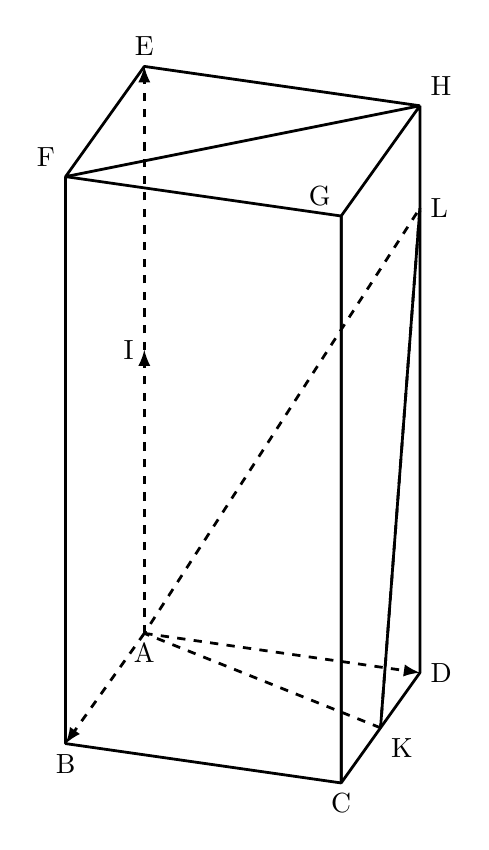
\begin{tikzpicture}[line width=1pt,line join=bevel,>=latex]
		%arêtes
		\draw (0.5,0.5)--(4,0)--(4,7.2)--(0.5,7.7)--cycle ; %BCGF
		\draw (4,0)--(5,1.4)--(5,8.6)--(4,7.2)--cycle ; %CDHG
		\draw (5,8.6)--(1.5,9.1)--(0.5,7.7)--cycle ; %HEF
		\draw[dashed,->] (1.5,1.9)--(1.5,5.5) ; %AI
		\draw[dashed,->] (1.5,1.9)--(0.5,0.5) ; %AB
		\draw[dashed,->] (1.5,1.9)--(5,1.4) ; %AD
		\draw[dashed,->] (4.5,0.7)--(1.5,1.9)--(5,7.3)--cycle ; %KAL
		\draw[dashed,->] (1.5,5.5)--(1.5,9.1) ;
		\draw (4.5,0.7)--(5,7.3) ;
		%labels
		\foreach \Point/\Nom/\Pos in {(0.5,0.5)/B/below,(4,0)/C/below,(4,7.2)/G/above left,(0.5,7.7)/F/above left,(5,1.4)/D/right,(5,8.6)/H/above right,(1.5,1.9)/A/below,(4.5,0.7)/K/below right,(1.5,5.5)/I/left,(5,7.3)/L/right,(1.5,9.1)/E/above}
		\draw \Point node[\Pos] {\Nom} ;
	\end{tikzpicture}
\end{center}

On se place dans le repère orthonormé $\left({A};\vect{{AB}},\vect{{AD}},\vect{{AI}}\right)$. 

On admet que le point $L$ a pour coordonnées $\left(0;1;\dfrac{3}{2}\right)$.

\begin{enumerate}
	\item Déterminer les coordonnées des vecteurs $\vect{{AK}}$ et $\vect{{AL}}$.
	\item 
	\begin{enumerate}
		\item Démontrer que le vecteur $\vect{n}$ de coordonnées $(6;-3;2)$ est un vecteur normal au plan $(AKL)$.
		\item En déduire une équation cartésienne du plan $(AKL)$.
		\item Déterminer un système d'équations paramétriques de la droite $\Delta$ passant par $D$ et
		perpendiculaire au plan $(AKL)$.
		\item En déduire que le point $N$ de coordonnées $\left(\dfrac{18}{49};\dfrac{40}{49};\dfrac{6}{49}\right)$ est le projeté orthogonal du point $D$ sur le plan $(AKL)$.
	\end{enumerate}
\end{enumerate}

On rappelle que le volume $\mathcal{V}$ d'un tétraèdre est donné par la formule : \[\mathcal{V} = \dfrac{1}{3}\times  (\text{aire de la base}) \times \text{hauteur}.\]
%
\begin{enumerate}[resume]
	\item 
	\begin{enumerate}
		\item Calculer le volume du tétraèdre $ADKL$ en utilisant le triangle $ADK$ comme base. 
		\item Calculer la distance du point $D$ au plan $(AKL)$.
		\item Déduire des questions précédentes l'aire du triangle $AKL$.
	\end{enumerate}
\end{enumerate}

